\chapter{Nuclear Physics}

\textit{Now I am become Death, the destroyer of worlds.}\\
\noindent\textbf{-    Bhagavad Gita}

\vspace{0.5cm}

\begin{marginfigure}[-10pt]
  
\includegraphics[width=\linewidth]{Nuclear_Family.jpg}
  \caption{Nuclear Family (DC Comics)}
  \label{fig:fig}
\end{marginfigure}

\vspace{0.5cm}

Nuclear physics starts with the discovery of radioactivity by Henri Becquerel in 1896, while investigating phosphorescence in uranium salts. The discovery of the electron by J. J. Thomson a year later was an indication that the atom had internal structure. 

At the beginning of the 20th century the accepted model of the atom was J. J. Thomson's "plum pudding" model in which the atom was a positively charged ball with smaller negatively charged electrons embedded inside it.  By 1900 physicists had also discovered three types of radiation emanating from atoms, which they named $\alpha$, $\beta$, and $\gamma$ radiation.  

By 1905, Albert Einstein formulated the idea of mass-energy equivalence. While the work on radioactivity by Becquerel and Marie Curie predates this, an explanation of the source of the energy of radioactivity would have to wait for the discovery that the nucleus itself was composed of smaller constituents, the nucleons.  In 1911 Rutherford scattering helped clarify the model of the atom as having a dense positively charged nucleus.
\marginnote[-150pt]{Satyendra Nath Bose was a Bengali physicist specializing in mathematical physics. He is best known for his work on quantum mechanics in the early 1920s, providing the foundation for Bose-Einstein statistics and the theory of the Bose-Einstein condensate.\\
Bose said Maxwell-Boltzmann distribution would not be true for microscopic particles, where fluctuations due to Heisenberg's uncertainty principle are significant. He theorized probability states in phase space having volumes $h^3$, disregarding the distinct position and momentum of particles.}
\vspace{0.5cm}

\section{Particles}

\begin{marginfigure}[0pt]
  \includegraphics[width=\linewidth]{bose.jpg}
  \caption{Satyendra Nath Bose}
  \label{fig:fig}
\end{marginfigure}

\begin{description}  
\item [Fermions]  Fermions are odd integer half spin particles.  They may be elementary particles or composite particles.  Fermions obey the Pauli exclusion principle, namely no two fermions can occupy the same quantum state.
\item [Bosons] Bosons are integer spin particles.  They may be elementary gauge bosons or composite particles.  Bosons obey Bose-Einstein statistics. Two bosons can occupy the same quantum state.  Cool bosons and they all condense into the ground state.
\item [Quarks]  Quarks are elementary particles and fundamental constituents of matter.  They have spin $\frac{1}{2}$ and are thus fermions.  Their charges are $\frac{2}{3}e$ or $-\frac{1}{3}e$.  There are six types of quarks, known as flavors: up, down, strange, charm, top, and bottom.  Antiquarks have opposite charge.
\begin{marginfigure}[0pt]
  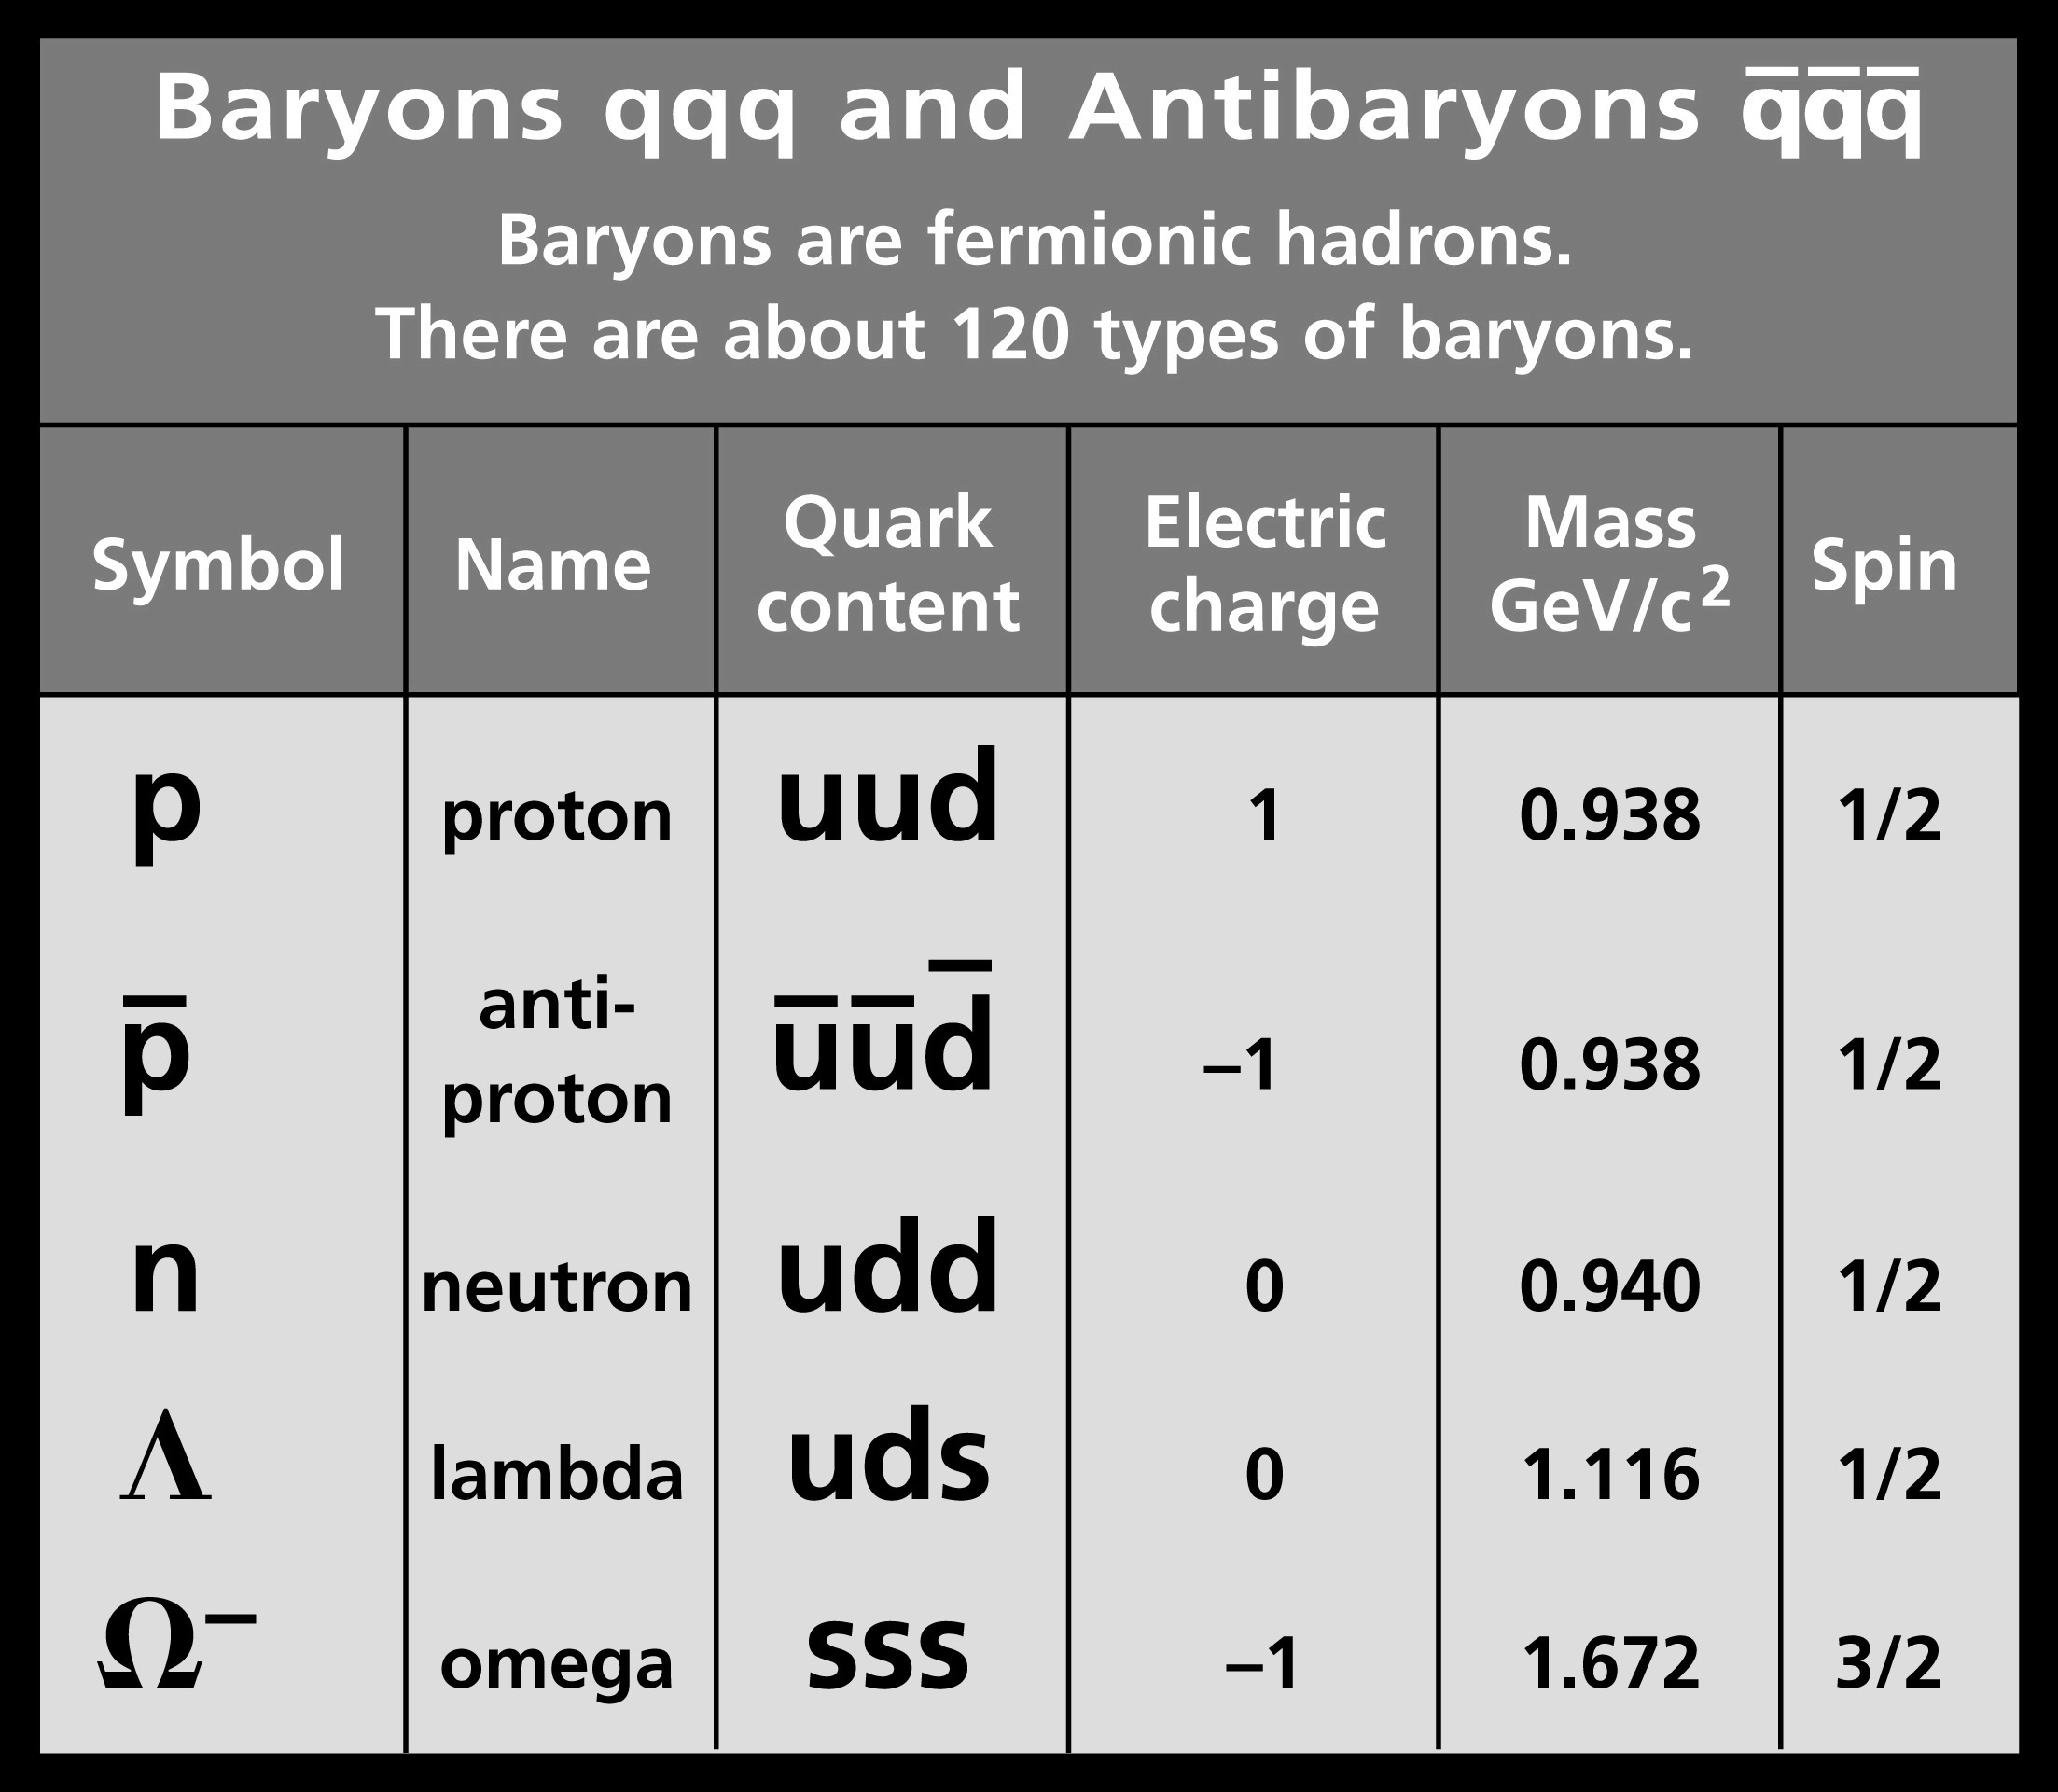
\includegraphics[width=\linewidth]{baryons.jpg}
  \caption{Baryons}
  \label{fig:fig}
\end{marginfigure}
\item [Hadrons]  Hadrons are clusters of quarks held together by the strong nuclear force.
\item [Baryons]  Baryons are triplet clusters of quarks.  They are fermions.  Nuclear particles such as protons and neutrons are baryons. 
\begin{marginfigure}[20pt]
  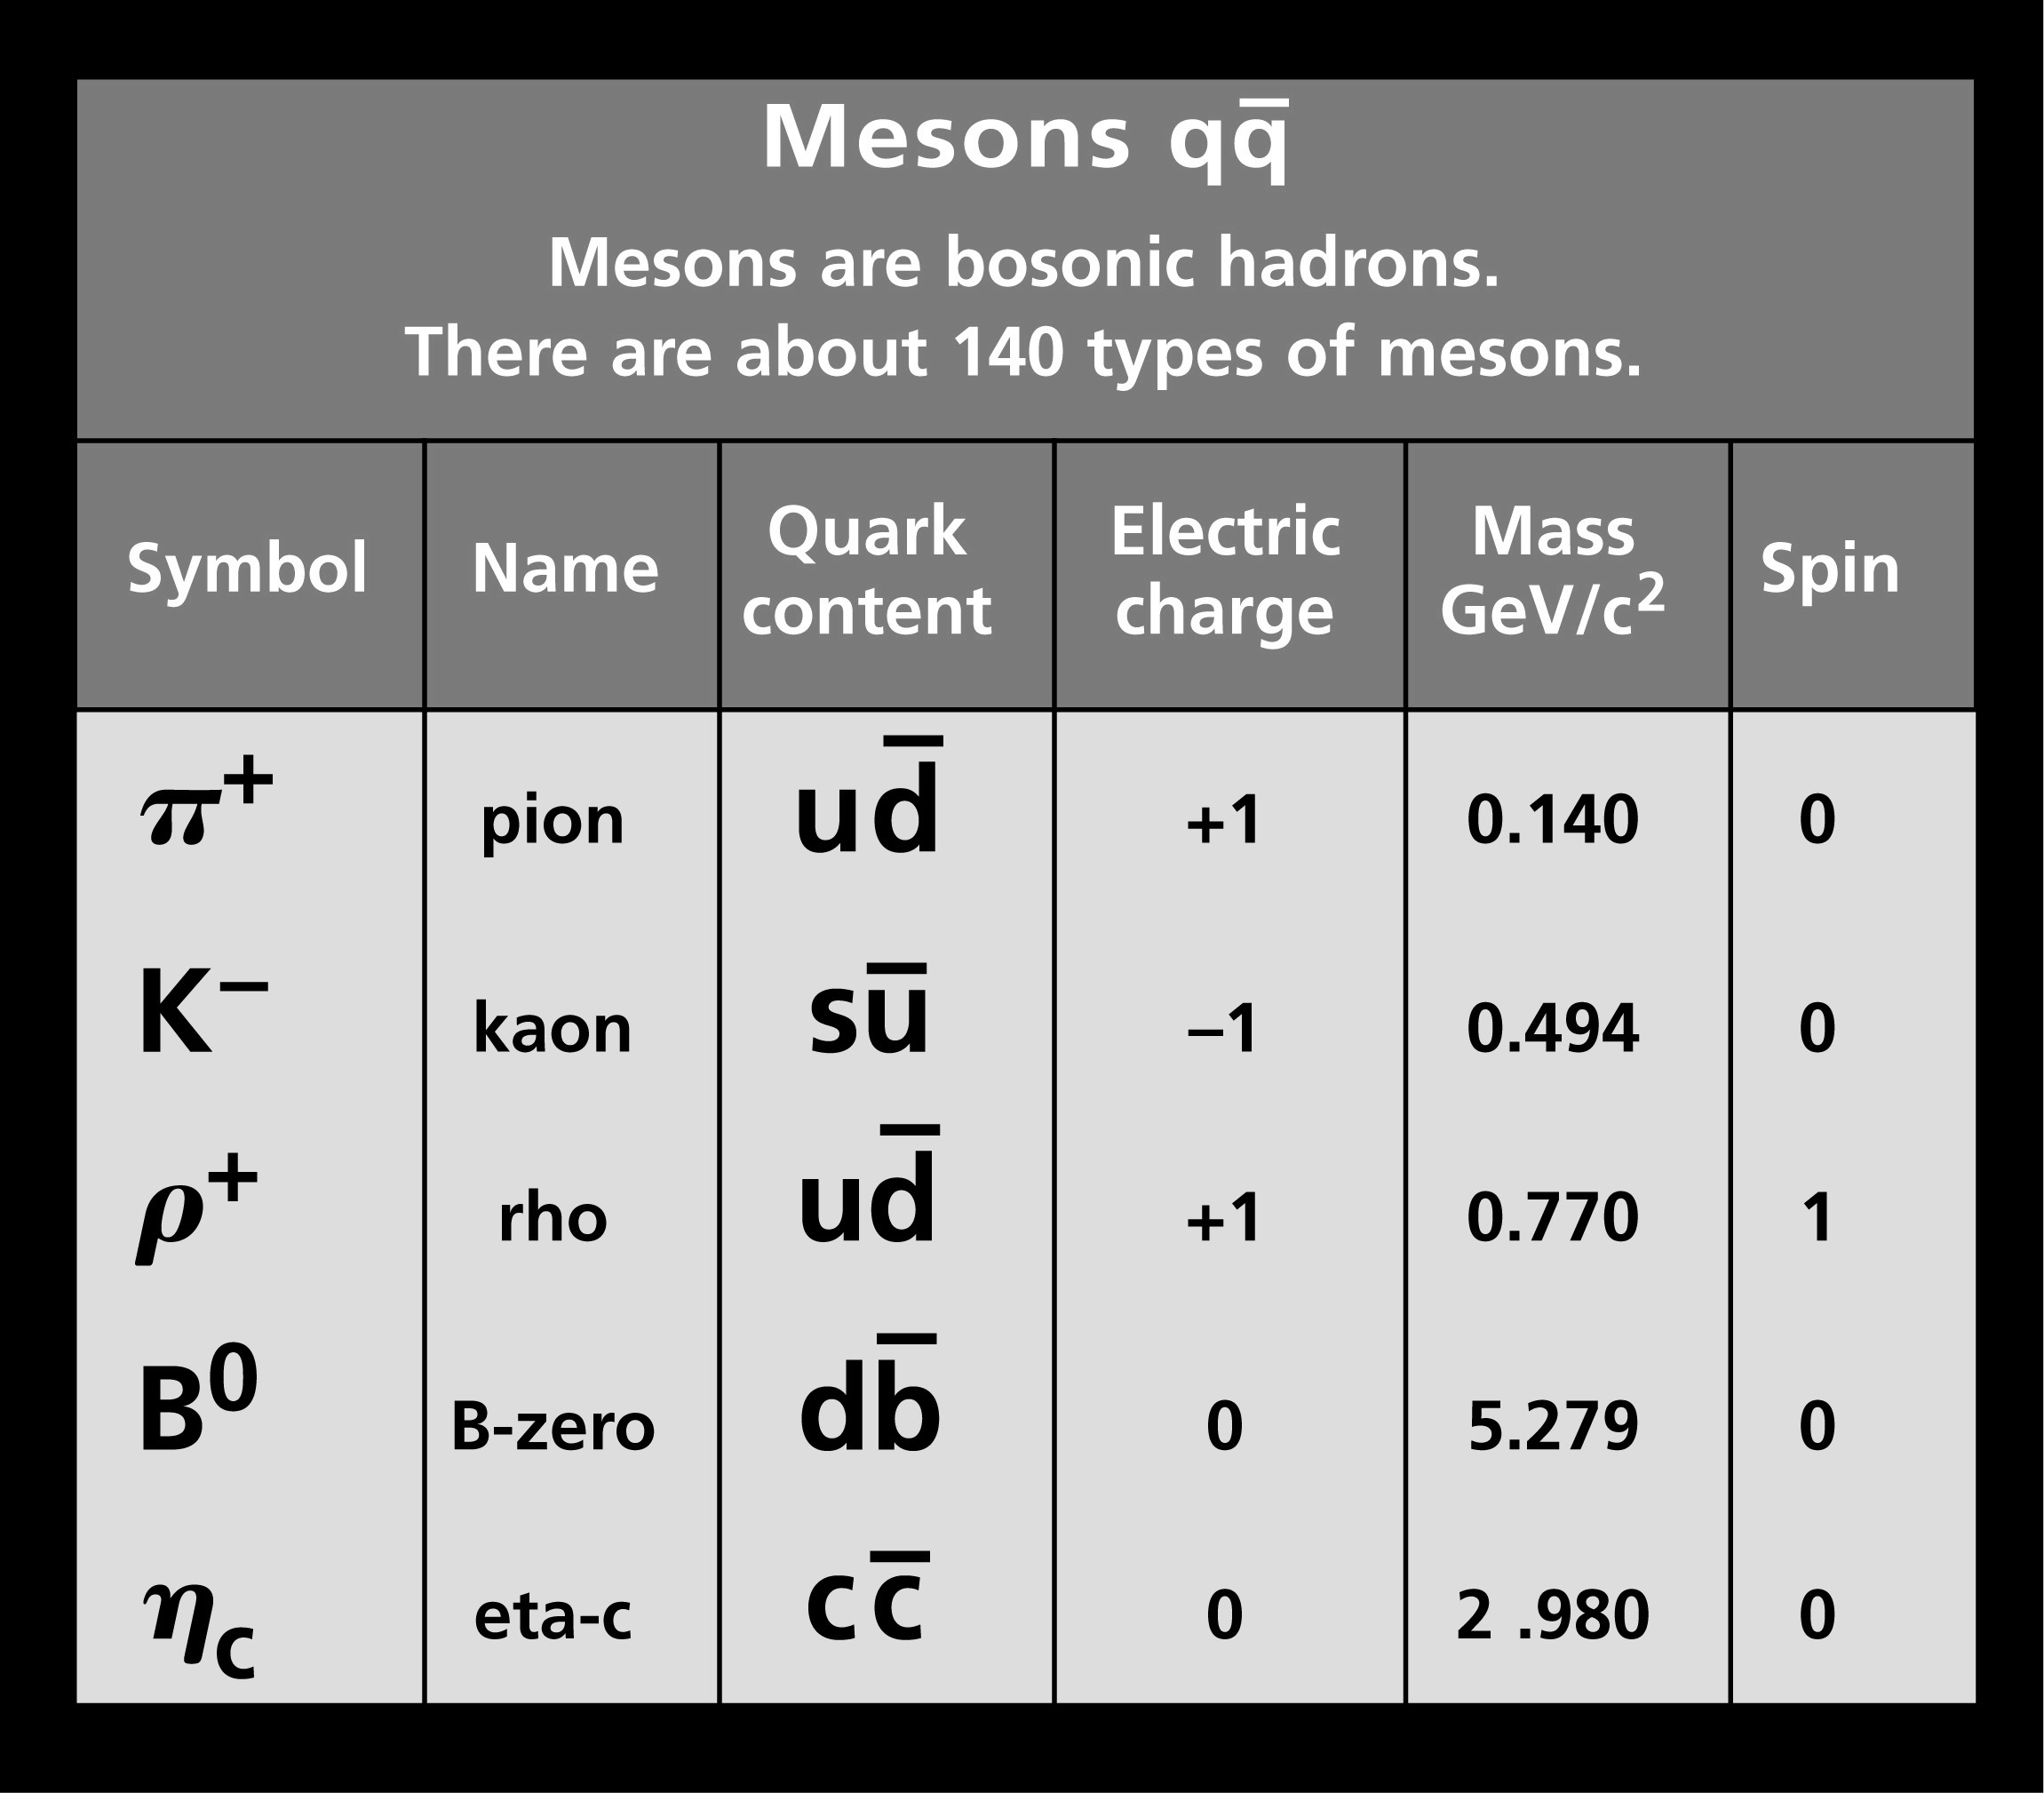
\includegraphics[width=\linewidth]{mesons.jpg}
  \caption{Mesons}
  \label{fig:fig}
\end{marginfigure}

\item [Mesons]  Mesons are hadronic particles composed of one quark and one antiquark.  All mesons are unstable, with the longest-lived lasting for only a few hundredths of a microsecond. 
\item [Leptons]  Leptons are elementary, half-integer spin particle that does not undergo strong interactions.  They are fermions. Two main classes of leptons exist: charged leptons (also known as the electron-like leptons), and neutral leptons (better known as neutrinos).
\item [Virtual Particles]  Virtual particles exchange one of the four fundamental forces of nature.  They are also known as exchange particles or gauge bosons.  They consist of photons (electromagnetic force), gluons (strong nuclear force), W and Z bosons (weak nuclear force) and gravitons (gravitational force).
\end{description}

\begin{figure}%
  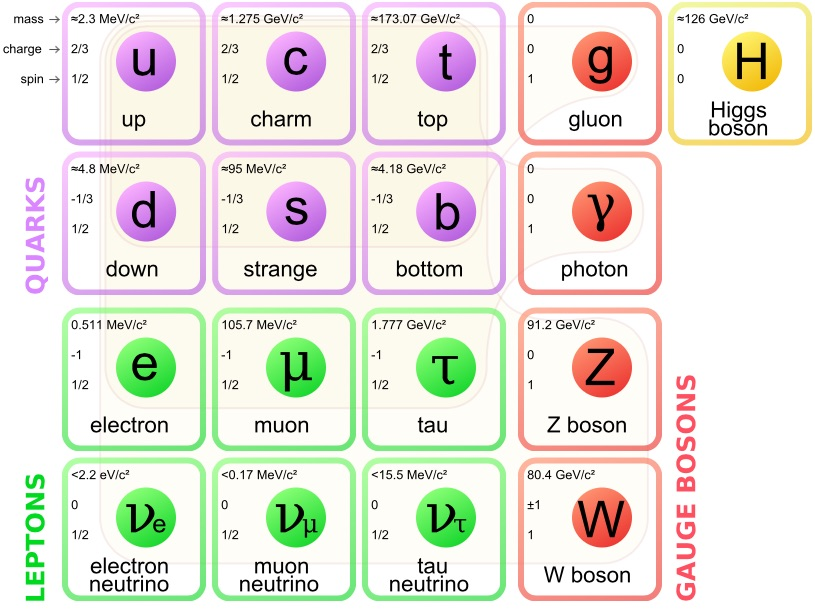
\includegraphics[width=\linewidth]{elem_particles.jpg}
  \caption{Particle Zoo}
  \label{fig:marginfig}
\end{figure}

\newpage
\section{Nuclear Decay}
\marginnote{For a given nucleus particle $A$ the number of baryons or nucleons (protons and neutrons) is $B$.  The charge of the particle is $C$.  For a nucleus $C$ is the number of protons while the number of neutrons is $B-C$.} 
 \marginnote[-20pt]{  \Huge $${}_{C}^{B}A$$}
  \marginnote[0pt]{  \subsection{Nucleons} Nucleons are baryons which constitute nuclear particles.  They are protons and neutrons.  They are approximately $10^{-15}$ meters in diameter and consist of up and down quarks held together by gluons.
  \subsubsection{Protons}
  Protons consist of two up quarks and one down quark.  Since the spin alignment of the two up quarks must be opposite the total spin of the proton is one half.  The total charge of the proton is $e$.
  \subsubsection{Neutrons}
  Nuetrons consist of two down quarks and one up quark.  Since the spin alignment of the down quarks must be opposite the total spin of the proton is one half.  The total charge of the neutron is zero.}
Radioactive decay, also known as nuclear decay or radioactivity, is the process by which the nucleus of an unstable atom loses energy by emitting radiation, including alpha particles, beta particles, gamma rays and conversion electrons. A material that spontaneously emits such radiation is considered radioactive.

Radioactive decay is a stochastic process at the level of single atoms, in that, according to quantum theory, it is impossible to predict when a particular atom will decay.  The chance that a given atom will decay never changes, that is, it does not matter how long the atom has existed. The decay rate for a large collection of atoms, however, can be calculated from their measured decay constants or half-lives. This is the basis of radiometric dating.
\subsection{Alpha Decay}
Alpha decay or $\alpha$-decay is a type of radioactive decay in which an atomic nucleus emits an alpha particle (helium-4 nucleus) and thereby transforms or decays into an atom with a mass number that is reduced by four and an atomic number that is reduced by two.  
Radium-226, for example, undergoes alpha decay to form radon-222.
$${}_{88}^{226}Ra \longrightarrow {}_{86}^{222}Rn +{}_{2}^{4}\alpha$$
\subsection{Beta Decay}
Beta decay ($\beta$-decay) is a type of radioactive decay in which a proton is transformed into a neutron, or vice versa, inside an atomic nucleus. This process allows the atom to move closer to the optimal ratio of protons and neutrons. As a result of this transformation, the nucleus emits a detectable particle, which is an electron $\beta^-$ or positron $\beta^+$.

Beta decay is mediated by the weak force. There are two types of beta decay.  In $\beta^-$ decay a neutron transmutes into a proton, producing an electron $e$ and an electron antineutrino $\bar{\nu}_e$.  In $\beta^+$ decay a proton transmutes into a neutron while a positron (anti-electron $\bar{e}$) and electron neutrino $\nu_e$ are produced.  $\beta^+$ decay is also known as positron emission.

$$\beta^-\  \text{decay:} \hspace{1cm} {}_{\ 6}^{14}C \longrightarrow {}_{\ 7}^{14}N +{}_{-1}^{\ 0}e + {}_{0}^{0}\bar{\nu}_e$$
$$\beta^+\  \text{decay:} \hspace{1cm}{}_{12}^{23}Mg \longrightarrow {}_{11}^{23}N +{}_{1}^{0}\bar{e} + {}_{0}^{0}\nu_e$$
\begin{marginfigure}[-50pt]
  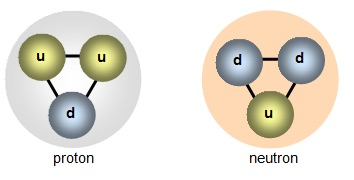
\includegraphics[width=\linewidth]{pro_neu.jpg}
  \caption{Protons and neutrons}
  \label{fig:fig}
\end{marginfigure}

\newpage

\begin{figure}%
  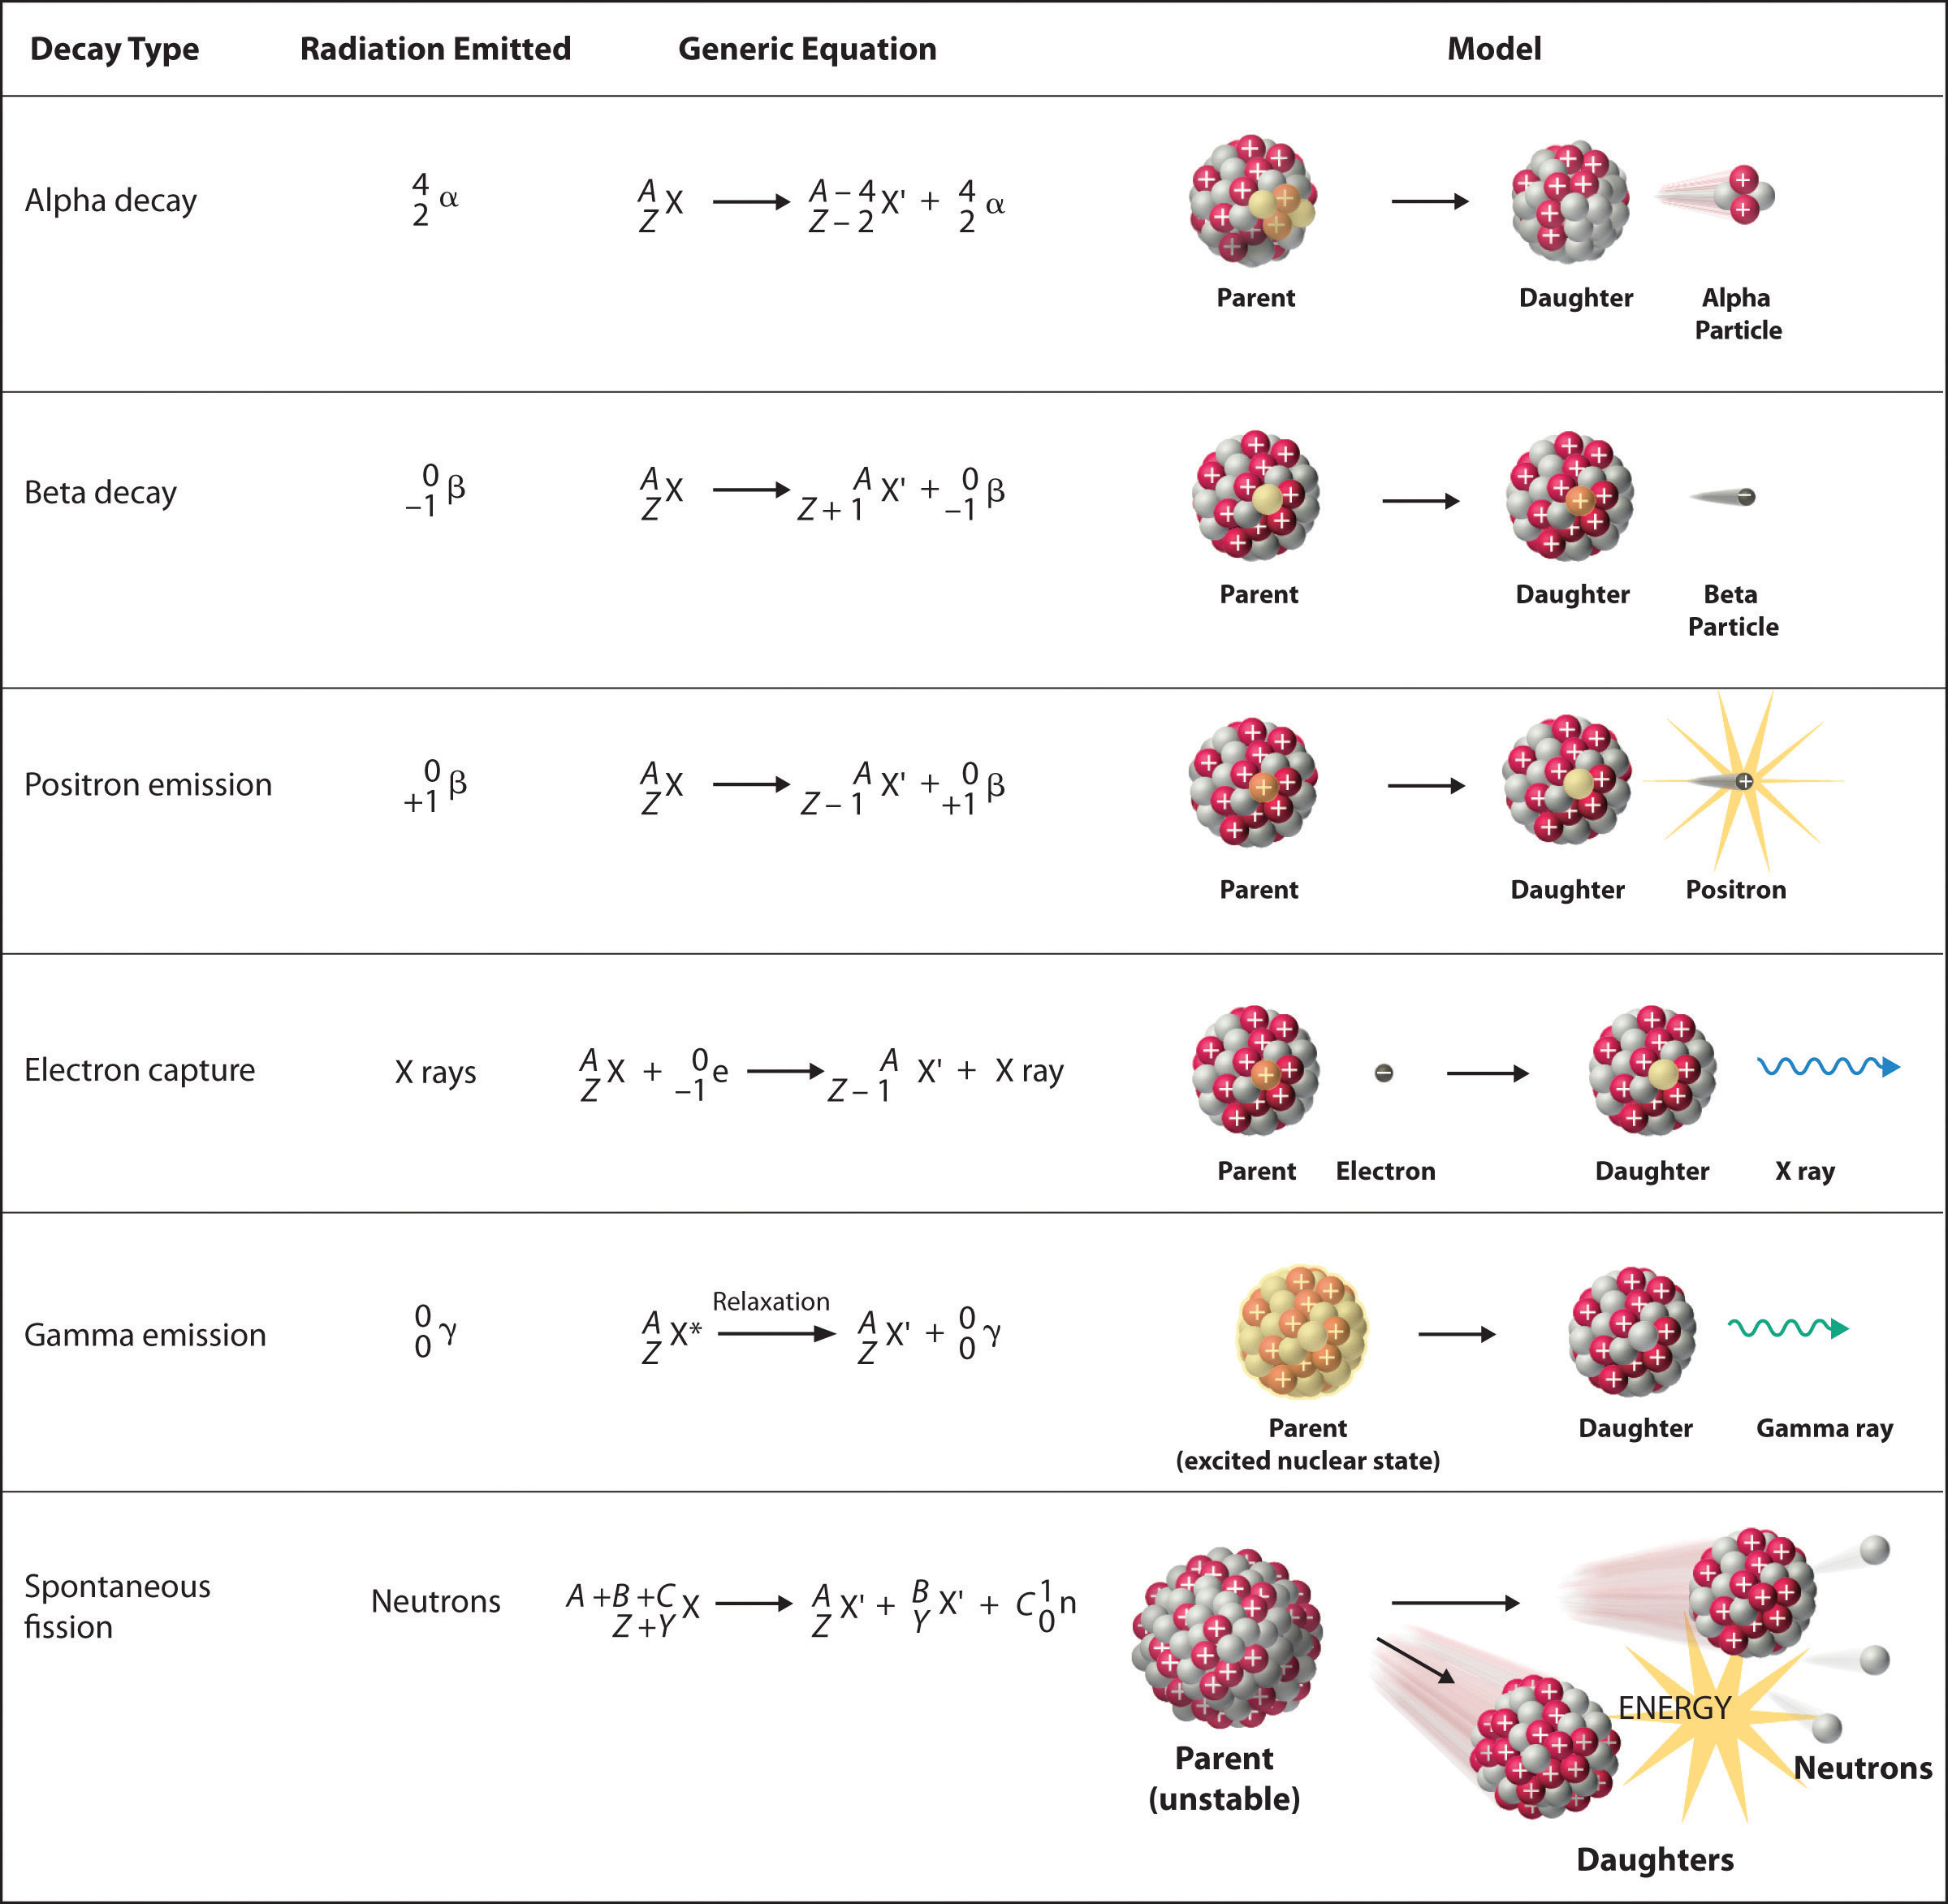
\includegraphics[width=\linewidth]{nuke_rxns.jpg}
  \caption{Nuclear decay reactions}
  \label{fig:marginfig}
\end{figure}
\marginnote[-300pt]{
\subsection{Strong Force}
Unlike gravity or electrical forces, the nuclear force is effective only at very short distances. At greater distances, the electrostatic force dominates: the protons repel each other because they are positively charged, and like charges repel.  The stability of the atomic nucleus requires at strong force with a different dependency on distance.

\subsection{Gamma Decay}
In gamma decay a nucleus changes from a higher energy state to a lower energy state through the emission of electromagnetic radiation (photons). The number of protons (and neutrons) in the nucleus does not change in this process, so the parent and daughter atoms are the same chemical element.

\subsection{Isotopes}
Isotopes are variants of a particular chemical element which differ in neutron number, although all isotopes of a given element have the same number of protons in each atom. The term isotope is formed from the Greek roots isos ("equal") and topos ("place"), meaning "the same place".  This means different isotopes of a single element occupy the same position on the periodic table.  Carbon-12, carbon-13 and carbon-14 are all isotopes of carbon.  They each have six protons but differeing number of neutrons.

\subsection{Units of Radioactivity}
The International System of Units (SI) unit of radioactive activity is the becquerel (Bq), named in honor of the scientist Henri Becquerel. One Bq is defined as one transformation (or decay or disintegration) per second.

An older unit of radioactivity is the curie, Ci, which was originally defined as "the quantity or mass of radium emanation in equilibrium with one gram of radium (element)".  Today, the curie is defined as $3.7\times10^{10}$ disintegrations per second, so that $1$ Ci = $3.7\times10^{10}$ Bq. }

\subsection{Exponential Decay and Half Life}
The decay rate for radioactive isotopes is proportional to the number of isotopes.  Here $N$ is the number of isotopes and $k$ is the decay rate constant.
$$\frac{\Delta N}{\Delta t}=-k N$$
This mathematical relationship describes a decaying exponential function.  Here $N_0$ is the intital number of particles.
$$N(t)=N_0 e^{-kt}$$
The half life $\tau_{1/2}$ of an isotope determines the time it takes for half a sample of that isotope to decay.  The half life is related to the decay constant $k$.
$$\tau_{1/2}=\frac{\ln 2}{k}$$
The decay function may be expressed in terms of the half life as follows.
$$N(t)=N_0 \left(\frac{1}{2}\right)^{\frac{t}{\tau_{\nicefrac{1}{2}}}}$$



\subsection{Fusion}
Nuclear fusion is a nuclear reaction in which two or more atomic nuclei fuse into a single nucleus. During this process, matter is not conserved because some of the matter of the fusing nuclei is converted to photons (energy). Fusion is the process that powers active or "main sequence" stars, or other high magnitude stars.
$${}_{1}^{2}H +{}_{3}^{6}Li\longrightarrow 2{}_{2}^{4}He $$


\begin{margintable}[0pt]\index{typefaces!sizes}
  \footnotesize%
  \begin{center}
    \begin{tabular}{clll}
      \toprule
     Z & Name & Symbol & Mass (amu) \\
      \midrule
     0    & Neutron & ${}^0n$ & 1.008664 \\
     1    & Hydrogen & ${}^1H$ & 1.007825 \\
           & Deuterium& ${}^2H$ & 2.014102 \\
           & Tritium & ${}^3H$ & 3.016049 \\
       2  & Helium & ${}^3He$ & 3.016029 \\
           &              & ${}^4He$ & 4.002603 \\
      3    & Lithium & ${}^6Li$ & 6.015122 \\
           &              & ${}^7Li$ & 7.016004 \\
      4   & Beryllium & ${}^9Be$ & 9.012182 \\
      5   & Boron & ${}^{10}B$ & 10.012937 \\
           &            & ${}^{11}B$ & 11.009305 \\
      6   & Carbon & ${}^{12}C$ & 12.000000 \\
                       &  & ${}^{13}C$ & 13.003355 \\
                      &  & ${}^{14}C$ & 14.003242 \\
      7   & Nitrogen & ${}^{14}N$ & 14.003074 \\
                     & & ${}^{15}N$ & 15.000109 \\
      8   & Oxygen & ${}^{16}O$ & 15.994915 \\
      & & ${}^{17}O$ & 16.999132 \\
      & & ${}^{18}O$ & 17.999160 \\
      9   & Fluorine & ${}^{19}F$ & 18.998403 \\
      10   & Neon & ${}^{20}Ne$ & 19.992440 \\
       & & ${}^{22}Ne$ & 21.991386 \\
      11 & Sodium & ${}^{23}Na$ & 22.989770 \\
      12   & Magnesium & ${}^{24}Mg$ & 23.985042 \\
        & & ${}^{25}Mg$ & 24.985837 \\
        & & ${}^{26}Mg$ & 25.982593 \\
      13   & Aluminum & ${}^{27}Al$ & 26.981538 \\
      14   & Silicon & ${}^{28}Si$ & 27.976927 \\
      15   & Phosphorus & ${}^{31}P$ & 30.973762 \\
      16   & Sulphur & ${}^{32}S$ & 31.972071 \\
      17   & Chlorine & ${}^{35}Cl$ & 34.968853 \\
      & & ${}^{37}Cl$ & 36.965903 \\
      18   & Argon & ${}^{37}Ar$ & 35.967546 \\
      &  & ${}^{40}Ar$ & 39.962383 \\
      19   & Potassium & ${}^{41}K$ & 40.961826 \\
      & & ${}^{40}K$ & 38.963707 \\
      20   & Calcium & ${}^{40}Ca$ & 39.962591 \\
      & & ${}^{44}Ca$ & 43.955481 \\
      21   & Scandium & ${}^{45}Sc$ & 44.955910 \\
      22  & Titanium & ${}^{46}Ti$ & 45.952629 \\
      &  & ${}^{48}Ti$ & 47.947947 \\
      23   & Vanadium & ${}^{50}V$ & 49.947163 \\
      & & ${}^{51}V$ & 50.943964 \\
      24   & Chromium & ${}^{50}Cr$ & 49.946050 \\
      &  & ${}^{52}Cr$ & 51.940512 \\
      25   & Manganese & ${}^{55}Mn$ & 54.938050 \\
      26   & Iron & ${}^{54}Fe$ & 53.939615 \\
      & & ${}^{56}Fe$ & 55.934942 \\
      & & ${}^{57}Fe$ & 56.935399 \\
      & & ${}^{58}Fe$ & 57.933280 \\
      27   & Cobalt & ${}^{59}Co$ & 58.933200 \\
      28   & Nickel & ${}^{58}Ni$ & 57.935348 \\ 
      & &${}^{60}Ni$ & 59.930791 \\ 
      & &${}^{61}Ni$ & 60.931060 \\ 
      & &${}^{62}Ni$ & 61.928349 \\ 
      & &${}^{64}Ni$ & 63.927970 \\    
      \bottomrule
    \end{tabular}
  \end{center}
  \caption{Light isotopes}
  \label{tab:font-sizes}
\end{margintable}

\subsection{Fission}
Nuclear fission is a radioactive decay process in which the nucleus of an atom splits into smaller parts. The fission process often produces free neutrons and gamma photons, and releases a very large amount of energy even by the energetic standards of radioactive decay.

$${}_{92}^{238}U \longrightarrow {}_{90}^{234}Th +{}_{2}^{4}He$$
\section{Mass Defect}
The mass defect of a nucleus is the difference between the mass of the nucleus and the mass of its constituent particles.  The mass of an atomic nucleus is usually less than the sum of the individual masses of the constituent protons and neutrons. This 'missing mass' is known as the mass defect. 
$${}_{2}^{4}He \longrightarrow 2{}_{1}^{1}H + 2{}_{0}^{1}n$$
$$4.002603 \longrightarrow 2(1.007825) + 2(1.008664)$$
$$\text{defect:}\hspace{1cm}\Delta m = 0.030375\ \text{u}$$

\section{Binding Energy}
Nuclear binding energy is the energy that would be required to disassemble the nucleus of an atom into its component parts.  The mass defect represents the mass equivalence of the binding energy.  
$$E=\Delta m c^2$$
The conversion factor between mass in atomic mass units and energy in mega electron volts is shown.
$$E=931.5\frac{\text{MeV}}{\text{u}}\ \Delta m$$
$${}_{2}^{4}He\ E_{bind}:\ \hspace{1cm}E=0.030375\ \text{u} \ \times \ 931.5\frac{\text{MeV}}{\text{u}}=28.29\text{MeV}$$
\newpage
\begin{figure}%
  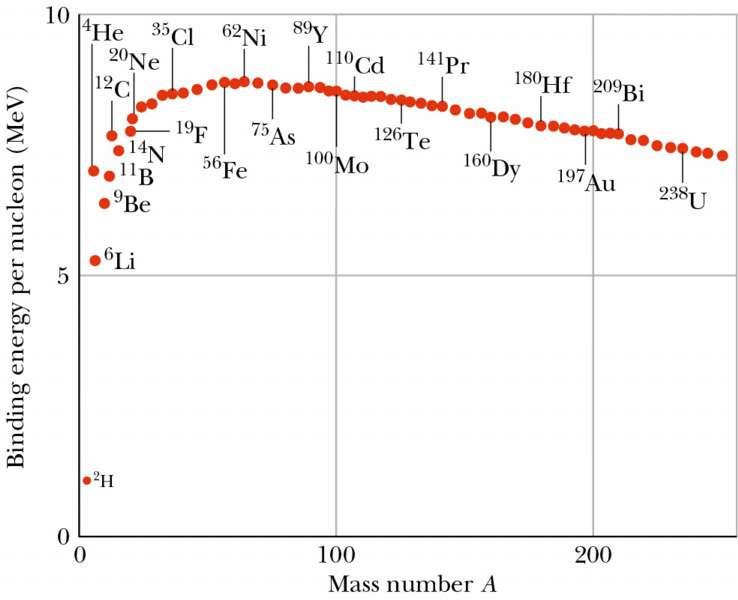
\includegraphics[width=\linewidth]{bindingE.jpg}
  \caption{Binding energy per nucleon}
  \label{fig:marginfig}
\end{figure}
\begin{margintable}[20pt]\index{typefaces!sizes}
  \footnotesize%
  \begin{center}
    \begin{tabular}{clll}
      \toprule
     Z & Name & Symbol & Mass (amu) \\
      \midrule
      29   & Copper & ${}^{63}Cu$ & 62.929601 \\
      30   & Zinc & ${}^{64}Zn$ & 63.929147 \\
      & & ${}^{64}Zn$ & 63.929147 \\
      & & ${}^{64}Zn$ & 63.929147 \\
      31   & Gallium & ${}^{69}Ga$ & 68.925581 \\
      & & ${}^{69}Ga$ & 68.925581 \\
      32   & Germanium & ${}^{70}Ge$ & 69.924250 \\
      & & ${}^{70}Ge$ & 69.924250 \\
      & & ${}^{70}Ge$ & 69.924250 \\
      33   & Arsenic & ${}^{75}As$ & 74.921596 \\
      34   & Selenium & ${}^{74}Se$ & 73.922477 \\
      & & ${}^{74}Se$ & 73.922477 \\
      & & ${}^{74}Se$ & 73.922477 \\
      35   & Bromine & ${}^{79}Br$ & 78.918338 \\
       & & ${}^{79}Br$ & 78.918338 \\
      36   & Krypton & ${}^{82}Kr$ & 81.913485 \\
      & & ${}^{83}Kr$ & 82.914136 \\
      & & ${}^{84}Kr$ & 83.911507 \\
      & & ${}^{86}Kr$ & 85.910610 \\
      & & ${}^{92}Kr$ & 91.926270 \\
      56   & Barium & ${}^{138}Ba$ & 137.905241 \\
      & & ${}^{141}Ba$ & 140.914411 \\
      80   & Mercury & ${}^{202}Hg$ & 201.970626 \\
      & & ${}^{206}Hg$ & 205.977514 \\
      81   & Thallium & ${}^{205}Tl$ & 204.974412 \\
      & & ${}^{206}Tl$ & 205.9761103 \\
      & & ${}^{207}Tl$ & 206.977419 \\
      & & ${}^{208}Tl$ & 207.9820187 \\
      & & ${}^{210}Tl$ & 209.990074 \\
      82   & Lead & ${}^{206}Pb$ & 205.9744653 \\
      & & ${}^{207}Pb$ & 206.9758969 \\
      & & ${}^{208}Pb$ & 207.976636 \\
      & & ${}^{210}Pb$ & 209.9841885 \\
      & & ${}^{214}Pb$ & 213.9998054 \\
      83   & Bismuth & ${}^{209}Bi$ & 208.980383 \\
      &  & ${}^{210}Bi$ & 209.9841204 \\
      &  & ${}^{214}Bi$ & 213.998712 \\
      84   & Polonium & ${}^{210}Po$ & 209.9828737 \\
      & & ${}^{214}Po$ & 213.9952014 \\
      & & ${}^{218}Po$ & 218.0089730 \\
      85   & Astatine & ${}^{210}At$ & 209.987131 \\
      86   & Radon & ${}^{222}Rn$ & 222.017570 \\
      87   & Francium & ${}^{223}Fr$ & 223.019731 \\
      88   & Radium & ${}^{226}Ra$ & 226.025403 \\
      89   & Actinium & ${}^{227}Ac$ & 227.027747 \\
      90   & Thorium & ${}^{230}Th$ & 230.0331338 \\
      & & ${}^{232}Th$ & 232.0380553 \\
      & & ${}^{234}Th$ & 234.043601 \\
      91   & Protactinium & ${}^{231}Pa$ & 231.035879 \\
      & & ${}^{234}Pa$ & 234.043308 \\
      99   & Uranium & ${}^{234}U$ & 234.040946 \\
       & & ${}^{235}U$ & 235.043923 \\
       & & ${}^{238}U$ & 238.050783 \\  
      \bottomrule
    \end{tabular}
  \end{center}
  \caption{Heavy isotopes}
  \label{tab:font-sizes}
\end{margintable}
\section{Binding Energy Per Nucleon}
Binding energy per nucleon is an important metric for determining the relative stability of isotopes.  Nuclei with the highest binding energy per nucleon are the most stable.  
A graph of binding energy per nucleon as a function of atomic mass number shows a trend of increasing binding energy per nucleon with larger nuclei up until the iron-56 and nickel-62.  The major exception is helium-4.  Carbon-12 is a minor exception.  
For nuclei larger then nickel-62 binding energy per nucleon goes down.  This means the larger nuclei are less stable.  In general elements lighter than iron-56 are candidates for fusion while elements heavier than nickel-62 are candidates for fusion.

$${}_{2}^{4}He\ \frac{E_{bind}}{\text{nucleon}}:\ \hspace{1cm}\frac{E}{\#N}=\frac{28.29\text{MeV}}{4}=7.07 \frac{\text{MeV}}{\text{nucleon}}$$

\section{Nuclear Reaction Energy}
To determine the energy of a nuclear reaction or decay process simply compare the mass of the products to the the mass of the reactants.  The difference in these two masses represents the energy of the reaction.

$${}_{1}^{2}H +{}_{3}^{6}Li\longrightarrow 2{}_{2}^{4}He $$
$$2.014102 +6.015122\longrightarrow 2(4.002603) $$
$$ \Delta m = 0.024018 \text{u}$$
$$E_{rxn}=0.024018 \text{u} \ \times \ 931.5\frac{\text{MeV}}{\text{u}}=22.37\text{MeV}$$


\begin{marginfigure}[60pt]
  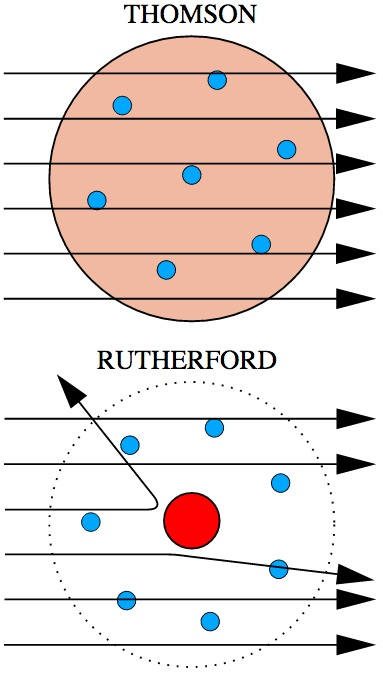
\includegraphics[width=0.8\linewidth]{scatter.jpg}
  \caption{Rutherford scattering}
  \label{fig:fig}
\end{marginfigure}

\section{Rutherford Scattering}
Rutherford scattering is the elastic scattering of charged particles by the Coulomb interaction. It is a physical phenomenon explained by Ernest Rutherford in 1911 that led to the development of the planetary Rutherford model of the atom and eventually the Bohr model.  Rutherford scattering was first referred to as Coulomb scattering because it relies only upon static electric (Coulomb) forces, and the minimal distance between particles is set only by this potential.

\subsection{Geiger-Mardsen Experiment}
The Geiger-Marsden experiment (also called the Rutherford gold foil experiment) indicated the existence of the nucleus where an atom's positive charge and most of its mass are concentrated. This was deduced this by measuring how an alpha particle beam is scattered when it strikes a thin metal foil.  
The experiment showed alpha particles bouncing off the metal foil in all directions, some right back at the source. This should have been impossible according to Thomson's model; the alpha particles should have all gone straight through. Obviously, those particles had encountered an electrostatic force far greater than Thomson's model suggested they would, which in turn implied that the atom's positive charge was concentrated in a much tinier volume than Thomson imagined.



